\documentclass{beamer}

\usepackage[utf8]{inputenc}
\usepackage{fancybox,fancyvrb}
\usepackage{environ}
\usepackage{tikz}

\beamertemplatenavigationsymbolsempty
\setbeamertemplate{footline}[frame number]
\setbeamertemplate{itemize item}{$\bullet$}
\setbeamertemplate{itemize subitem}{$\circ$}

\newcommand{\grad}{\nabla}
\newcommand{\ih}{\boldsymbol{\hat{\textbf{\i}}}}
\newcommand{\jh}{\boldsymbol{\hat{\textbf{\j}}}}


\title{2.4 Exact (first-order differential) Equations}

\subtitle{a lesson for MATH F302 Differential Equations}

\author{Ed Bueler, Dept.~of Mathematics and Statistics, UAF}

\date{\tiny \today}


\usetheme{Pittsburgh}


\begin{document}


\begin{frame}
\titlepage

\centerline{\tiny for textbook: \, D. Zill, \emph{A First Course in Differential Equations with Modeling Applications}, 11th ed.}
%\color{green!40!blue}
\end{frame}


\begin{frame}{two objects from calculus III}

to get started on exact equations we recall these two ideas:
\begin{enumerate}
\item \begin{minipage}[t]{0.4\textwidth}
\emph{vector fields}:
    $$\boldsymbol{\vec{\textbf{F}}} = a(x,y) \ih + b(x,y) \jh$$
\end{minipage}
\begin{minipage}[t]{0.5\textwidth}
\vspace{-2mm}

\hfill 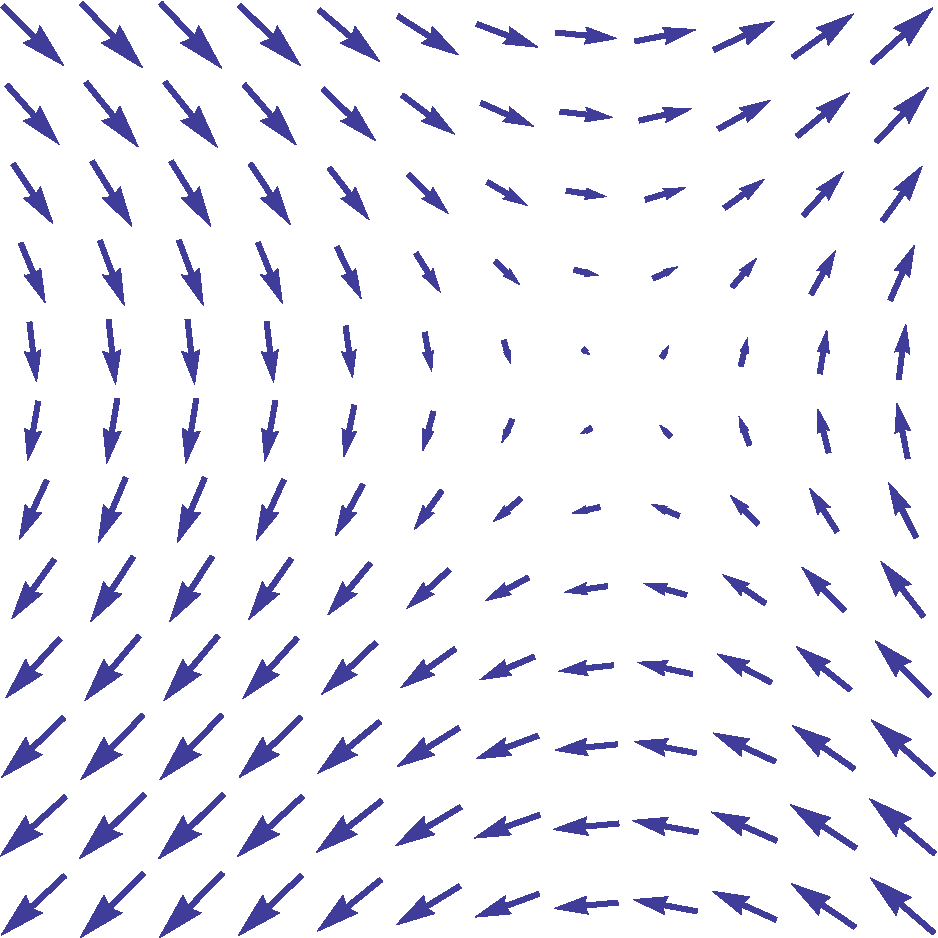
\includegraphics[width=0.5\textwidth]{figs/VectorField}

\hfill \tiny $\boldsymbol{\vec{\textbf{F}}} = \sin y \ih + \sin x \jh$
\end{minipage}

\vspace{-4mm}
\item the \emph{gradient} of a function $f(x,y)$:
    $$\grad f(x,y) = \frac{\partial f}{\partial x} \ih + \frac{\partial f}{\partial y} \jh$$
    \begin{itemize}
    \item the gradient \emph{is} a vector field:  $a=\frac{\partial f}{\partial x}$, $b=\frac{\partial f}{\partial y}$
    \item the gradient points uphill on the surface $z=f(x,y)$
    \item the \emph{differential} of $f$, namely $df = \frac{\partial f}{\partial x}\,dx + \frac{\partial f}{\partial y}\,dy$, contains the same information as the gradient
    \end{itemize}
\end{enumerate}
\end{frame}


\begin{frame}{a biggish idea}

\begin{itemize}
\item note we will need to be able to compute partial derivatives!
\item \emph{big idea}: some vector fields are the gradients of an $f$ and some are not
    \begin{itemize}
    \item Example 1: FIXME
    \item Example 2: FIXME
    \end{itemize}
\item \emph{same big idea}: some differential forms
    $$M(x,y)\,dx + N(x,y)\,dy$$
are the differentials of an $f$---they're \alert{exact}---and some are not
\end{itemize}
\end{frame}


\begin{frame}{X}

\begin{itemize}
\item X
\end{itemize}
\end{frame}


\begin{frame}{expectations}

to learn this material, just watching this video is \emph{not} enough; also
\begin{itemize}
\item \emph{watch} ``found online'' videos at

\centerline{\href{https://bueler.github.io/math302/week4.html}{\tt \color{cyan} bueler.github.io/math302/week4.html}}
\item \emph{try-out} Euler's method codes at the same link
\item \emph{read} section 2.4 in the textbook
\item \emph{do} the WebAssign exercises for section 2.4
\end{itemize}
\end{frame}

\end{document}

